\documentclass[12pt]{article}
\usepackage{fullpage}
\usepackage{lastpage}
\usepackage{fancyhdr}
\pagestyle{fancy}

\addtolength{\topmargin}{-0.25in}
\usepackage{graphicx, caption}	
\usepackage{array, multicol, tabu}
\usepackage{amsmath}
\usepackage{comment}
\usepackage{enumerate}
\usepackage{url}
\usepackage{textcomp}
\newcommand{\vect}[1]{\mathbf{#1}}
%\everymath{\displaystyle}

\fancypagestyle{plain}{
	\fancyhf{}
	\addtolength{\headheight}{2.92\baselineskip}
	\lhead{\bf MATH 2554 (Calculus I) \\
		Spring 2016 \\
		}
	\rhead{{Name:} \underline{\hspace{40ex}} \\
		\vspace{0.5pc}
		Fri 8 Apr 2016}
	\rfoot{Exam 3 p.\thepage\ (of \pageref{LastPage})}
	}
\fancyhf{}
\renewcommand{\headrulewidth}{0pt}

\title{\vspace{-8pc}
\vfill{\Huge
	\bf Exam 3: Applications and Story Problems (\S 3.10-4.6)} 
	}
\author{}
\date{}

\rfoot{Exam 3 p.\thepage\ (of \pageref{LastPage})}

\begin{document}
\maketitle
%\vfill
\vspace{-3pc}
\noindent{\bf Exam Instructions:} You have 50 minutes to complete this exam.  Justification is required for all problems.  Notation matters!  You will also be penalized for missing units and rounding errors.  No electronic devices (phones, iDevices, computers, etc) except for a \textbf{basic scientific calculator}.  On story problems, round to one decimal place. %If you finish early then you may leave, UNLESS there are less than 5 minutes of class left.  To prevent disruption, if you finish with less than 5 minutes of class remaining then please stay seated and quiet.

\begin{flushright}
In addition, please provide the following data:

\vspace{1.5pc}
Drill Instructor: \underline{\hspace{40ex}}

\vspace{1.5pc}
Drill Time: \underline{\hspace{40ex}}
\end{flushright}

%\vspace{2pc}
\vfill
\noindent\textbf{Your signature below indicates that you have read this page and agree to follow the Academic Honesty Policies of the University of Arkansas.}  

\vspace{2pc}
\noindent Signature: {\bf (1 pt)} \underline{\hspace{73ex}}

%\vfill
\begin{flushright}\Large Good luck!\end{flushright}

\begin{enumerate}[1.]
% % % % % % % % % %	

\newpage 

% % %
\item %{\bf 4.6 (5 min)}
\begin{enumerate}\item {\bf(5 pts)} Explain why Rolle's Theorem cannot be applied to the function $f(x)=|x|$ on the interval $[-a,a]$ for any $a>0$.
\vspace{5pc}

\item {\bf(3 pts)} Is there any interval where Rolle's Theorem applies to $f(x)$?  Why or why not?
\vspace{5pc}

\item {\bf(3 pts)} Is there any interval where the Mean Value Theorem applies to $f(x)$?  Why or why not?
\vspace{5pc}
\end{enumerate}

% % %
\item %{\bf 4.4} 
{\bf(12 pts)} Suppose you own a tour bus and you book groups of 20 to 70 people for a day tour.  The cost per person is \$30 minus 25\textcent\ for every ticket sold.  If gas and other miscellaneous costs are \$200, how many tickets should you sell to maximize your profit?
\vspace{20pc}

% % %
%\item {\bf 4.6}
%Determine whether the Mean Value Theorem applies for each of the given functions.  If it does, then find the point(s) guaranteed by the theorem to exist.
%\begin{enumerate}
%	\item {\bf (3 min)} $f(x)=3\sin{2x}$ on $[0,\frac{\pi}{4}]$
%	\vspace{20pc}
%	
%	\item {\bf (3 min)} $f(x)=x+\frac{1}{x}$ on $[1,3]$
%	\vspace{20pc}
%\end{enumerate}

% % %
\newpage
\item %{\bf 4.5} %3.7} 
%Let $g(x)=\frac{x}{x+1}$.
%Let $f(x)=\sin{x}$ and $g(x)=\cos{x}$.
	\begin{enumerate}	\item {\bf(3 pts)} Write the equations for the linear approximation to $g(x)=\sin x$ and $h(x)=\cos x$ at $x=0$.
	\begin{align*}
	\sin x \approx & \hspace{300pt}\\[0.5pc]
	\cos x \approx &	
	\end{align*}
	\vspace{12pc}
	\item {\bf(3pts)} Use your answers to (a) to approximate $\sin{(0.1)}$ and $\cos{(0.1)}$.

	\vspace{6pc}
	\item {\bf(5 pts)} The following are the respective graphs of $\sin x$ and $\cos x$, drawn at the website \url{desmos.com/calculator}.  On each graph, draw your tangent line.  Label both your approximations from (b) and the exact values $\sin{(0.1)}$ and $\cos{(0.1)}$.  
	
	\vspace{2pc}
	\centering{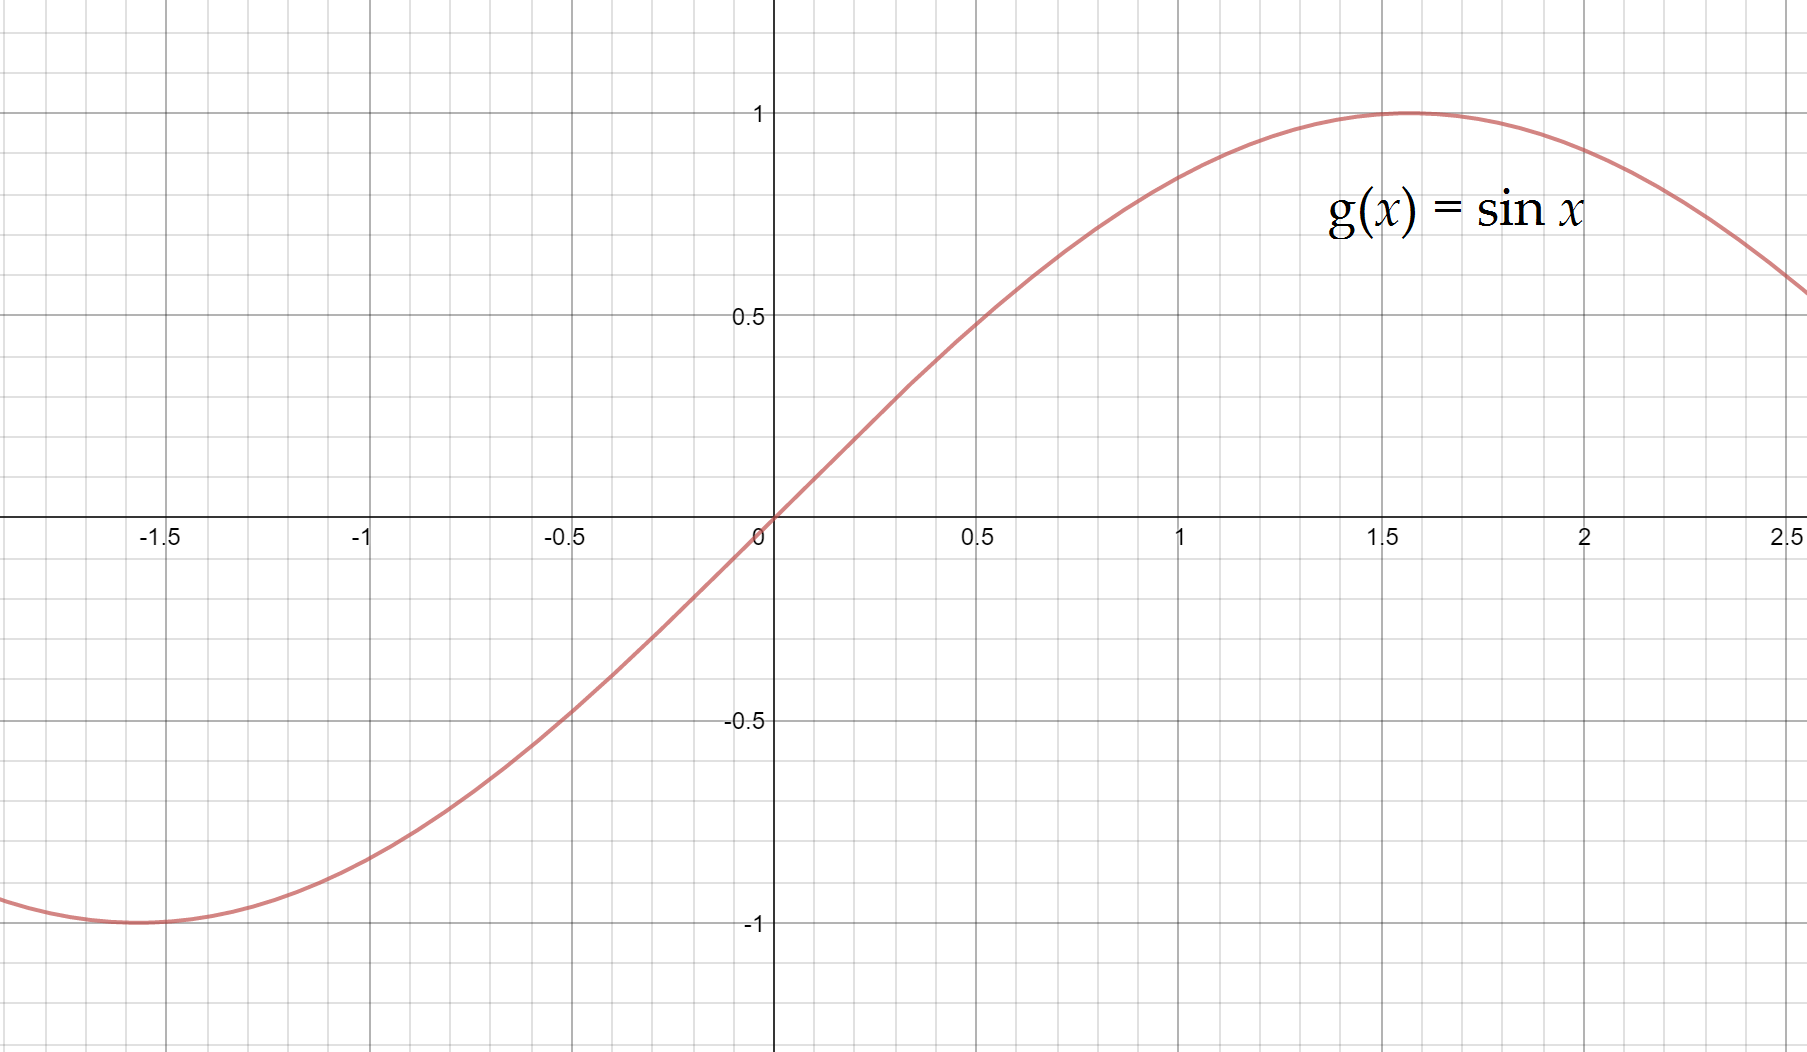
\includegraphics[scale=0.53]{exam3LinApproxSin}}
		
	\vspace{2pc}
	\centering{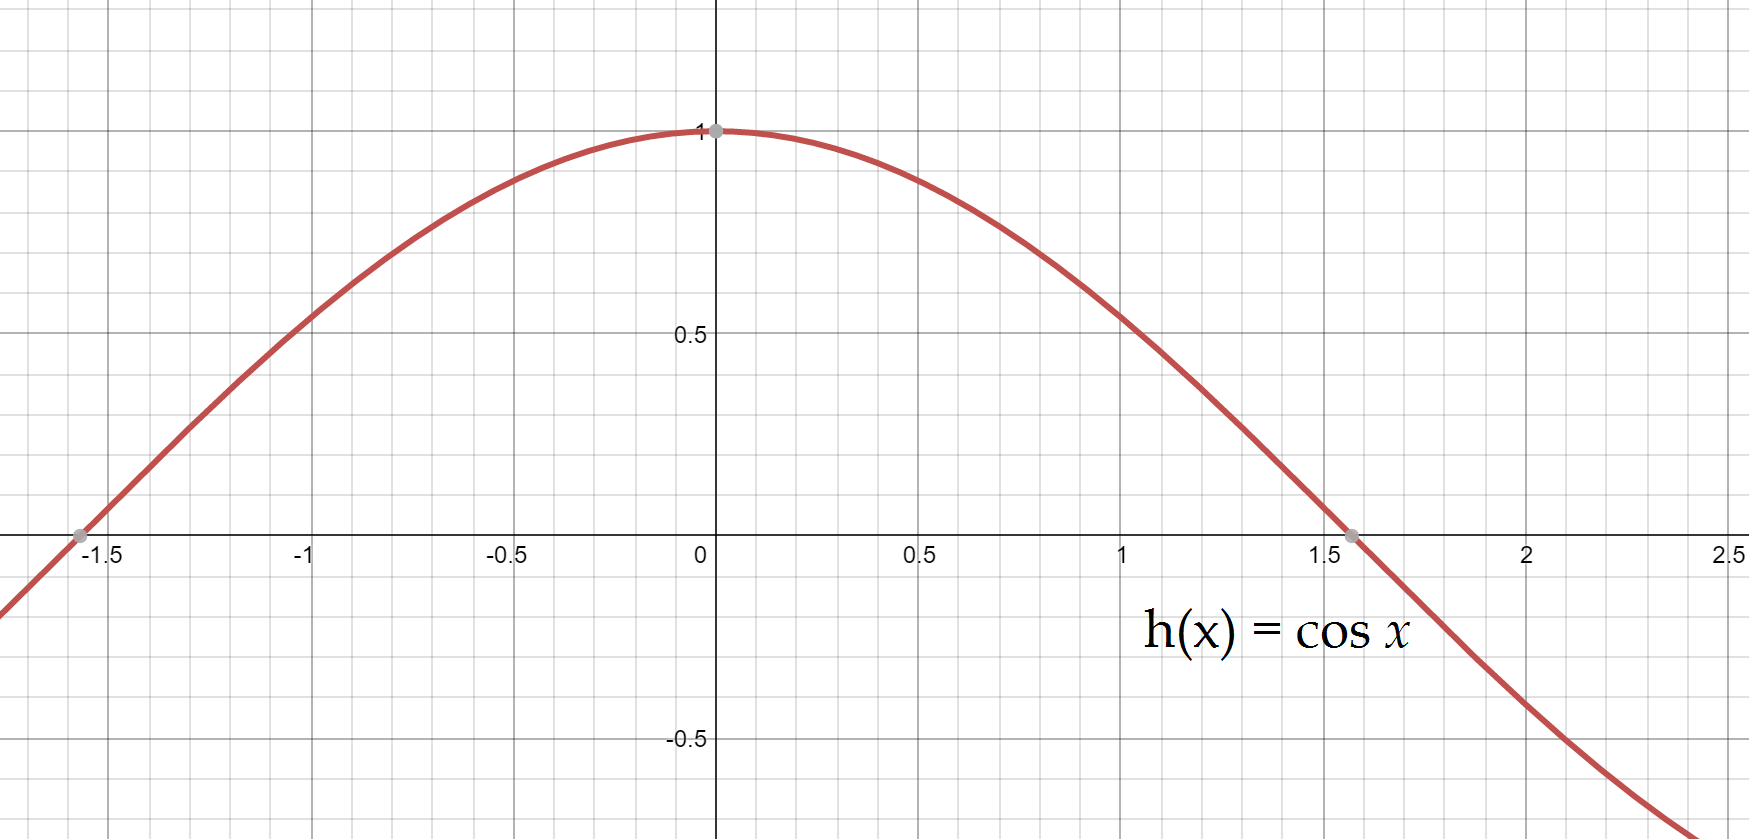
\includegraphics[scale=0.55]{exam3LinApproxCos}}
	\end{enumerate}

\vspace{1pc}
\item %{\bf 3.11} %(3.8 H 5 min)} 
{\bf(12 pts)} Two cylindrical swimming pools are being filled simultaneously at the same rate (in m$^{\text{3}}$/min).  The smaller pool has a radius of 5m, and the water level rises at a rate of 0.5m/min.  The larger pool has a radius of 8m.  How fast is the water level rising in the larger pool?

% % % % %
\newpage
% % %
\item %{\bf 3.10, 4.1-4.3} 
The goal of this problem is to produce a graph of the function
\[f(x)=\tan^{-1}{x^3}\]
from scratch.
	
	\begin{enumerate}
	\item {\bf (2 pts)} Find the domain for $f(x)$.
	
	\vspace{8pc}
	\item {\bf (2pts)} Is $f(x)$ even, odd, or neither?  You must justify your answer.
	
	\vspace{10pc}
	\item {\bf (4 pts)} Find $f'(x)$ and $f''(x)$.  You are not required to simplify.
	
	% %
	\newpage
	%\vspace{10pc}
	\item {\bf (3 pts)} Find the critical points.  If there are none, then say why.
	
	% %
	%\newpage
	\vspace{10pc}
	\item {\bf (3 pts)} Find the possible inflection points.  If there are none, then say why.
	
	\vspace{10pc}
	\item {\bf (3 pts)} What are the intervals where $f(x)$ is increasing?  What are the intervals where $f(x)$ is decreasing?
	
	% %
	\newpage
	%\vspace{10pc}
	\item {\bf (3 pts)} What are the intervals where $f(x)$ is concave up?  What are the intervals where $f(x)$ is concave down?
	
	% %
	%\newpage
	\vspace{23pc}
	\item {\bf (4 pts)} Find the local extrema and inflection points.  You must justify your answers.  If there are no extrema or inflection points you should also say why.
	
	% %
	\newpage
	%\vspace{12pc}
	%\item {\bf (2 pts)} Find the vertical asymptotes, using the limit definition of a vertical asymptote.  If there are no vertical asymptotes, then say so.
	
	%\vspace{14pc}
	%\item {\bf (2 pts)} Determine the end behavior.  
	
	% %
	\newpage
	%\vspace{20pc}
	%\item {\bf (2 pts)} Find the $y$-intercepts and $x$-intercepts, if there are any.  
	
	% %
	%\newpage
	\vspace{18pc}
	\item {\bf (4 pts)} Use all the information above, plus the following facts, to draw a well-labeled graph of $f(x)$.  Your picture should be consistent with your answers to (a)-(h).
	\begin{itemize}
	\item $f(x)$ has no vertical asymptotes, but it has horizontal asymptotes at $y=\pm\frac{\pi}{2}$.
	\item $f(x)$ intersects the origin.
	\end{itemize}
	\end{enumerate}

% % % % % % % % % %
\end{enumerate}
\end{document}


